%! TEX program = xelatex
\documentclass{beamer}

%%% Usepackage
% Basic
\usepackage{xeCJK}     % Chinese support
\usepackage{amsmath}   % Math input support
\usepackage{amssymb}   % Math input support
\usepackage{booktabs}  % 3 line table show
\usepackage{float}     % Figure and Table env.
\usepackage{makecell}  % Mult. lines in one table cell

% Color Support
\usepackage{xcolor}
\definecolor{commcolor}{rgb}{0,0.6,0}
\definecolor{rulesepcolor}{rgb}{0.2,0.2,0.2}
\definecolor{stringcolor}{rgb}{0.58,0,0.82}
\definecolor{backcolor}{rgb}{0.93,0.87,0.89}
\definecolor{backcolor2}{rgb}{1,1,0.9}

% Coding block
\usepackage{listings}
\lstset{
  language=python,
  basicstyle=\tiny\ttfamily,
  captionpos=b,
  backgroundcolor=\color{backcolor2},
  commentstyle=\color{commcolor},
  escapeinside={\%*}{*)},
  keywordstyle=\color{blue},
  stringstyle=\color{stringcolor}\ttfamily,
  frame=none,
  rulesepcolor=\color{rulesepcolor},
  numbers=left,
  numbersep=4pt,
  numberstyle={\color[RGB]{170,170,170}},
  % xleftmargin=1.5em,
  % xrightmargin=1.5em,
}

% Coding block smooth
\usepackage{tikz}
\usepackage[framemethod=tikz,skipbelow=\topskip,skipabove=\topskip]{mdframed}
\mdfsetup{
  leftmargin=0pt,
  rightmargin=0pt,
  backgroundcolor=backcolor2,
  middlelinecolor=backcolor2,
  roundcorner=5pt,
}
\usepackage{etoolbox}
\BeforeBeginEnvironment{lstlisting}{\begin{mdframed}\vspace{-1em}}
\AfterEndEnvironment{lstlisting}{\vspace{-1em}\end{mdframed}}

% Inline coding
\usepackage{newverbs}
\newverbcommand{\cverb}
  {\setbox\verbbox\hbox\bgroup}
  {\egroup\tcbox{\color{purple}\box\verbbox}}

% Picture shadow box & Inline coding bg
\usepackage[many]{tcolorbox}
\tcbset{
  on line,
  boxsep=0.6pt, 
  left=0pt, right=0pt, top=0pt, bottom=0pt,
  colframe=backcolor, 
  colback=backcolor,  
  highlight math style={enhanced}
}


%%% New command
\newcommand{\purple}{\textcolor{purple}}


%%% Page style
\setbeamertemplate{navigation symbols}{}
\usefonttheme{professionalfonts}
\usetheme{Madrid}
\usecolortheme{default}


%%% Pages
%+===================================================================+%
\title[CMT.Tsinghua]{如何写好一个数据处理程序}
\subtitle{(Python入门简介)}

\author[Yang Li]{
  李洋 (Yang Li)\inst{1}}  
\institute[Physics@Tsinghua]{
  \inst{1} Department of Physics\\
           Tsinghua University 
}

\date[Tsinghua Physics 2021]{May. 2021}
%-===================================================================-%

%+===================================================================+%
\AtBeginSection[]
{
  \begin{frame}
    \frametitle{目录}
    \tableofcontents[currentsection]
  \end{frame} 
}
%-===================================================================-%
 
\begin{document}
  %+===================================================================+%
  \frame{\titlepage}
  %-===================================================================-%

  %+===================================================================+%
  \begin{frame}[fragile]{前置声明}
    \begin{block}{内容声明}
      以下所有内容都是笔者参考自身编程经验总结得到, 或许某些论点会出现认知或表述上的错误. 还请大家批判性地接受.
    \end{block}
    \begin{block}{版权声明}
      本Slides内容发布在GitHub上, 并受\cverb|GPL-3.0|开源许可证保护. 您可以自由的下载、复用、修改其中内容, 并进一步作为它用. 他人修改再发布版本与本作者无关.\\
      {\tiny \purple{\url{https://github.com/kYangLi/PublicPresentation/blob/master/AcaCode/latex-src/main.pdf}}}
    \end{block}
  \end{frame}
  %-===================================================================-%

  %+===================================================================+%
  \begin{frame}
    \frametitle{目录}
    \tableofcontents
  \end{frame}
  %-===================================================================-%

  \section{为什么需要编程?}
    %+===================================================================+%
    \begin{frame}{编程的本质}
      \begin{block}{编程的定义}
        所谓编程, 其实就是\purple{使用计算机语言, 实现人与计算机间有效交流的手段}, 是让计算机理解并执行``人想进行的复杂操作"的媒介. 计算机语言之所以称之为``语言'', 是因为他确实有一般语言的特性, 即, 他是一种约定俗成的, 可以被两个独立个体分别无信息损失地理解的记号. 在有些时候, 编程语言也成为了人与人之间交流算法和感情的基本语言.
      \end{block}
      \begin{block}{高级计算机语言的特点}
        \begin{itemize}
          \item 语法要求非常严密, 有时写错一个符号就会导致整体 代码无法运行.
          \item 结构十分规整, 一段优秀的代码天然会具有层次分明的结构美感.
          \item 起源于英语, 并与英语表达有相似之处. 一段优秀的代码会使阅读代码者产生阅读英文概述的错觉.
          \item 种类繁多, 特性各异.
        \end{itemize}
      \end{block}
      \textcolor{gray}{真正控制了世界的, 其实是程序员们.}
    \end{frame}
    %-===================================================================-% 

    %+===================================================================+%
    \begin{frame}{编程应用1: 实验仪器的数据采集(串口通讯)}
      \begin{columns}
        \begin{column}{0.8\textwidth}
          \centering
          \begin{tcolorbox}[beamer,width=0.8\textwidth,arc=0pt,boxsep=0pt,left=0pt,right=0pt,top=0pt,bottom=0pt]
            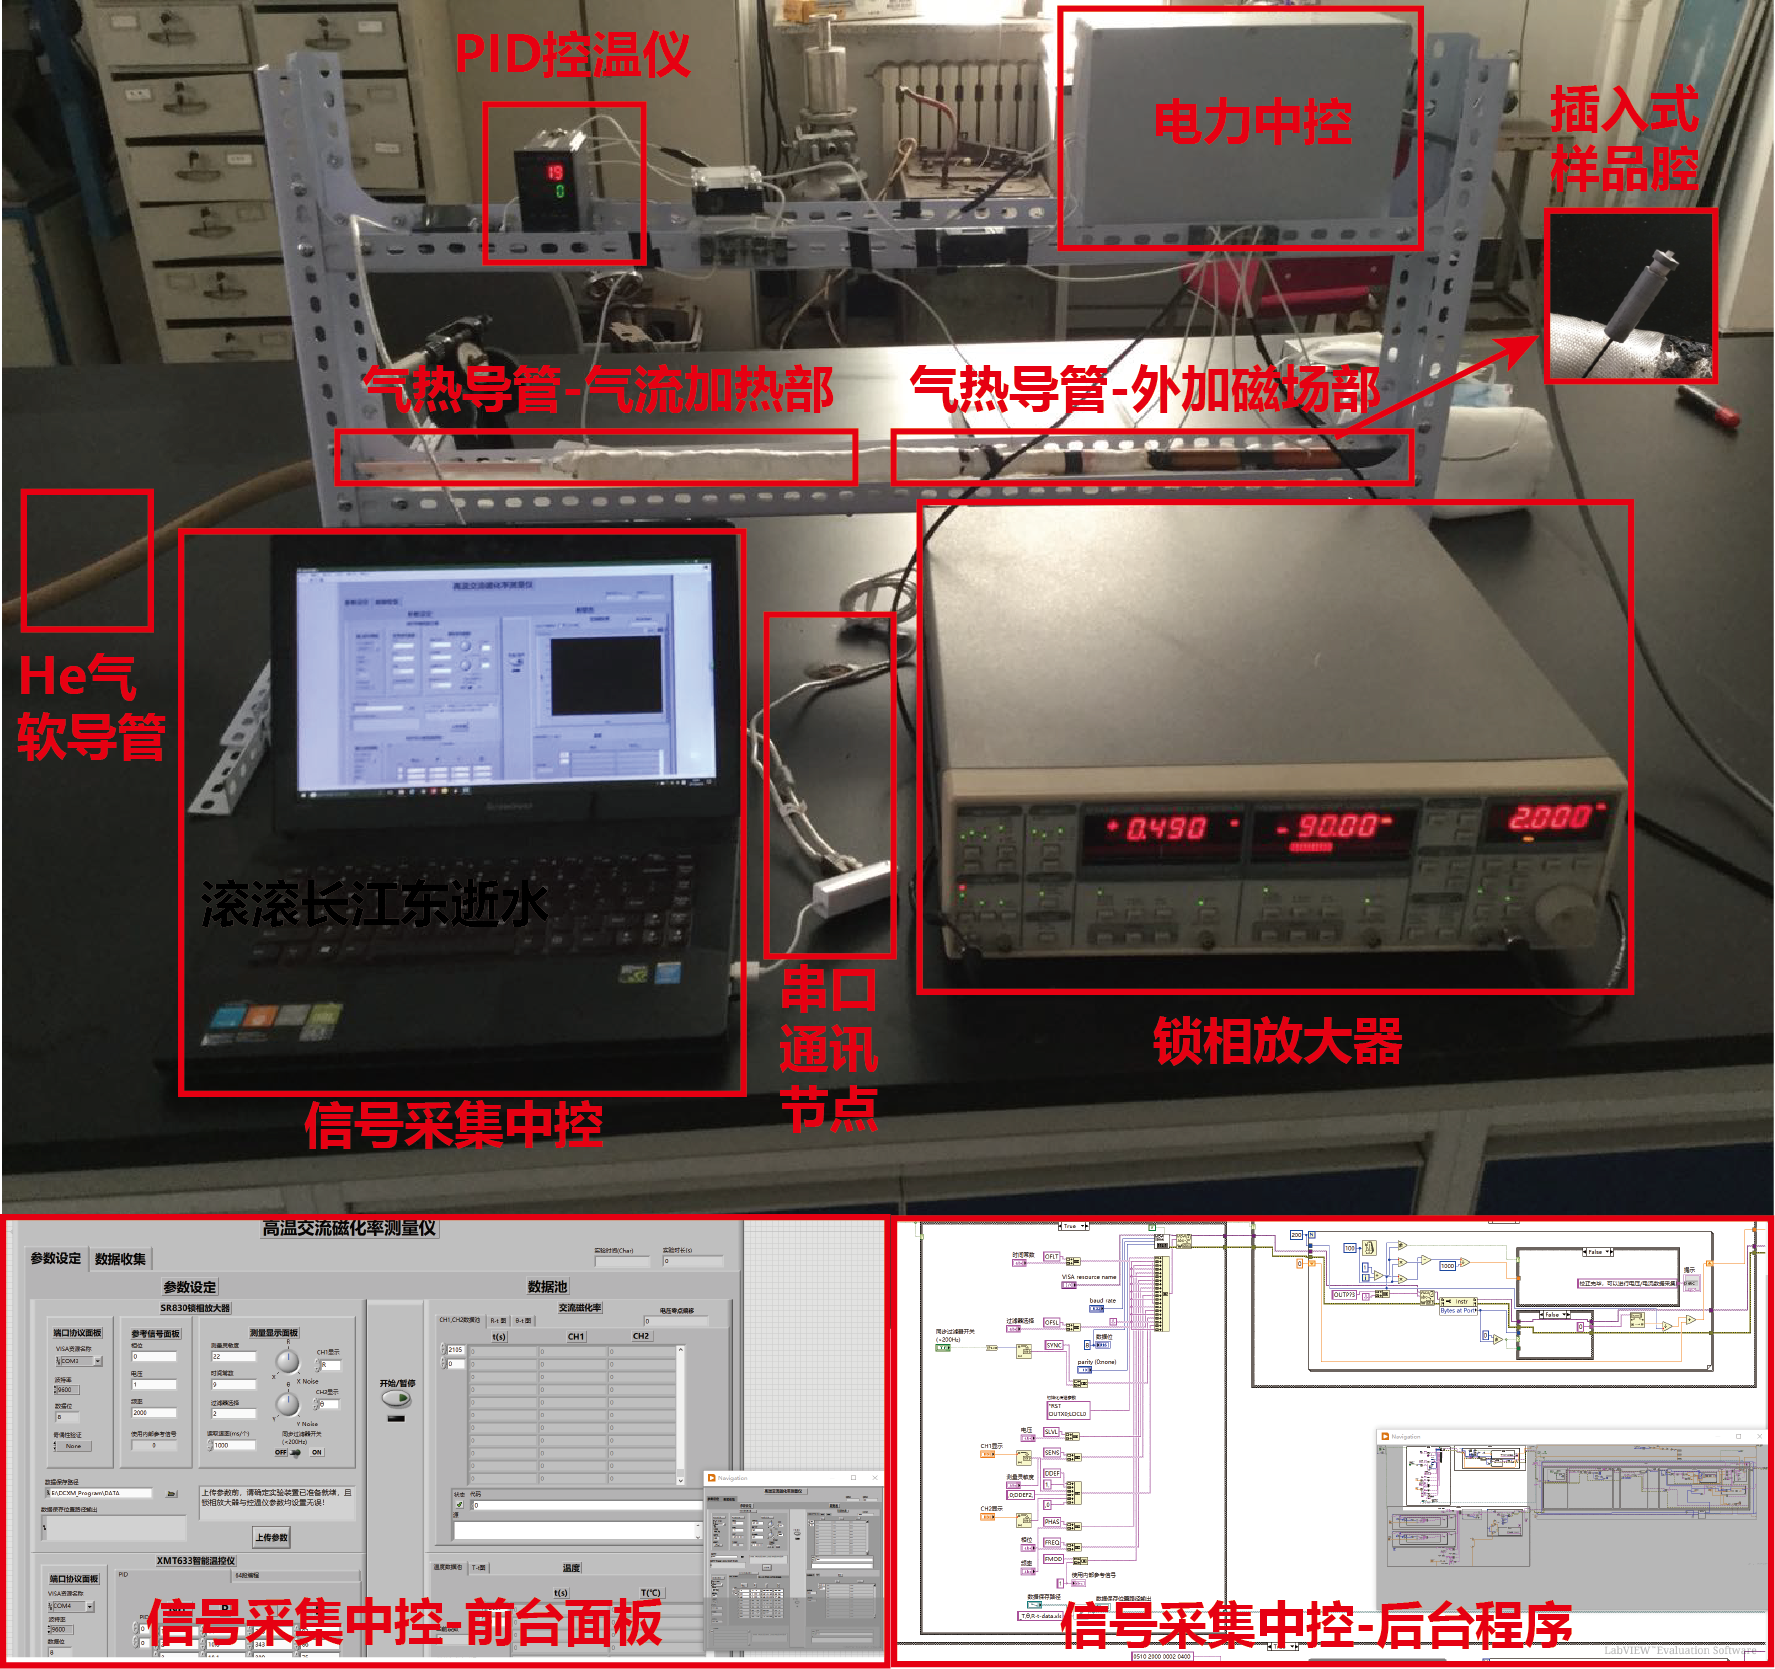
\includegraphics[width=\textwidth]{figure/dc.png}
          \end{tcolorbox}
        \end{column}
        \begin{column}{0.16\textwidth}
          \centering
          \begin{block}{}\small
            各种各样的传感器和信号采集设备规范化了实验的进行. 信号采集和数据处理完全需要依靠相关语言, 如LabVIEW中的G语言, 编程实现. 
          \end{block}
        \end{column}
        \begin{column}{0.1\textwidth}
        \end{column}
      \end{columns}
    \end{frame}
    %-===================================================================-%

    %+===================================================================+%
    \begin{frame}{编程应用2: 实验数据峰值拟合}
      \begin{columns}
        \begin{column}{0.85\textwidth}
          \centering
          \begin{tcolorbox}[beamer,width=0.88\textwidth,arc=0pt,boxsep=0pt,left=0pt,right=0pt,top=0pt,bottom=0pt]
            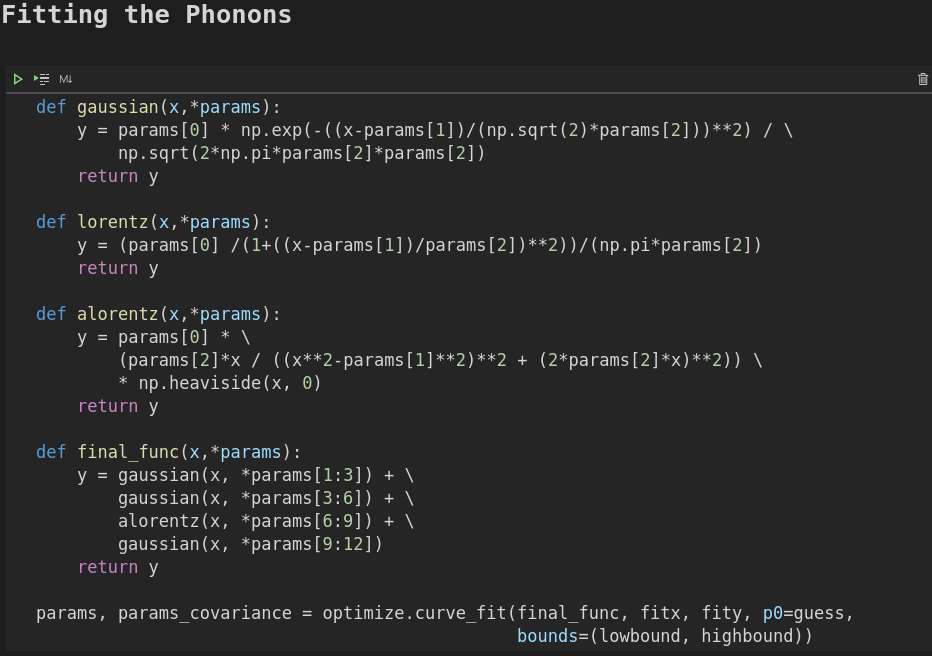
\includegraphics[width=\textwidth]{figure/curv-fitting.png}
          \end{tcolorbox}
        \end{column}
        \begin{column}{0.16\textwidth}
          \centering
          \begin{block}{}
            实验的后续数据处理, 如寻找实验信号中的峰值和模式匹配时一般也需要编程实现.
          \end{block}
        \end{column}
        \begin{column}{0.1\textwidth}
        \end{column}
      \end{columns}
    \end{frame}
    %-===================================================================-%

    %+===================================================================+%
    \begin{frame}{编程应用3: 流程化VASP第一原理计算}
      \centering
      \begin{tcolorbox}[beamer,width=\textwidth,arc=0pt,boxsep=0pt,left=0pt,right=0pt,top=0pt,bottom=0pt]
        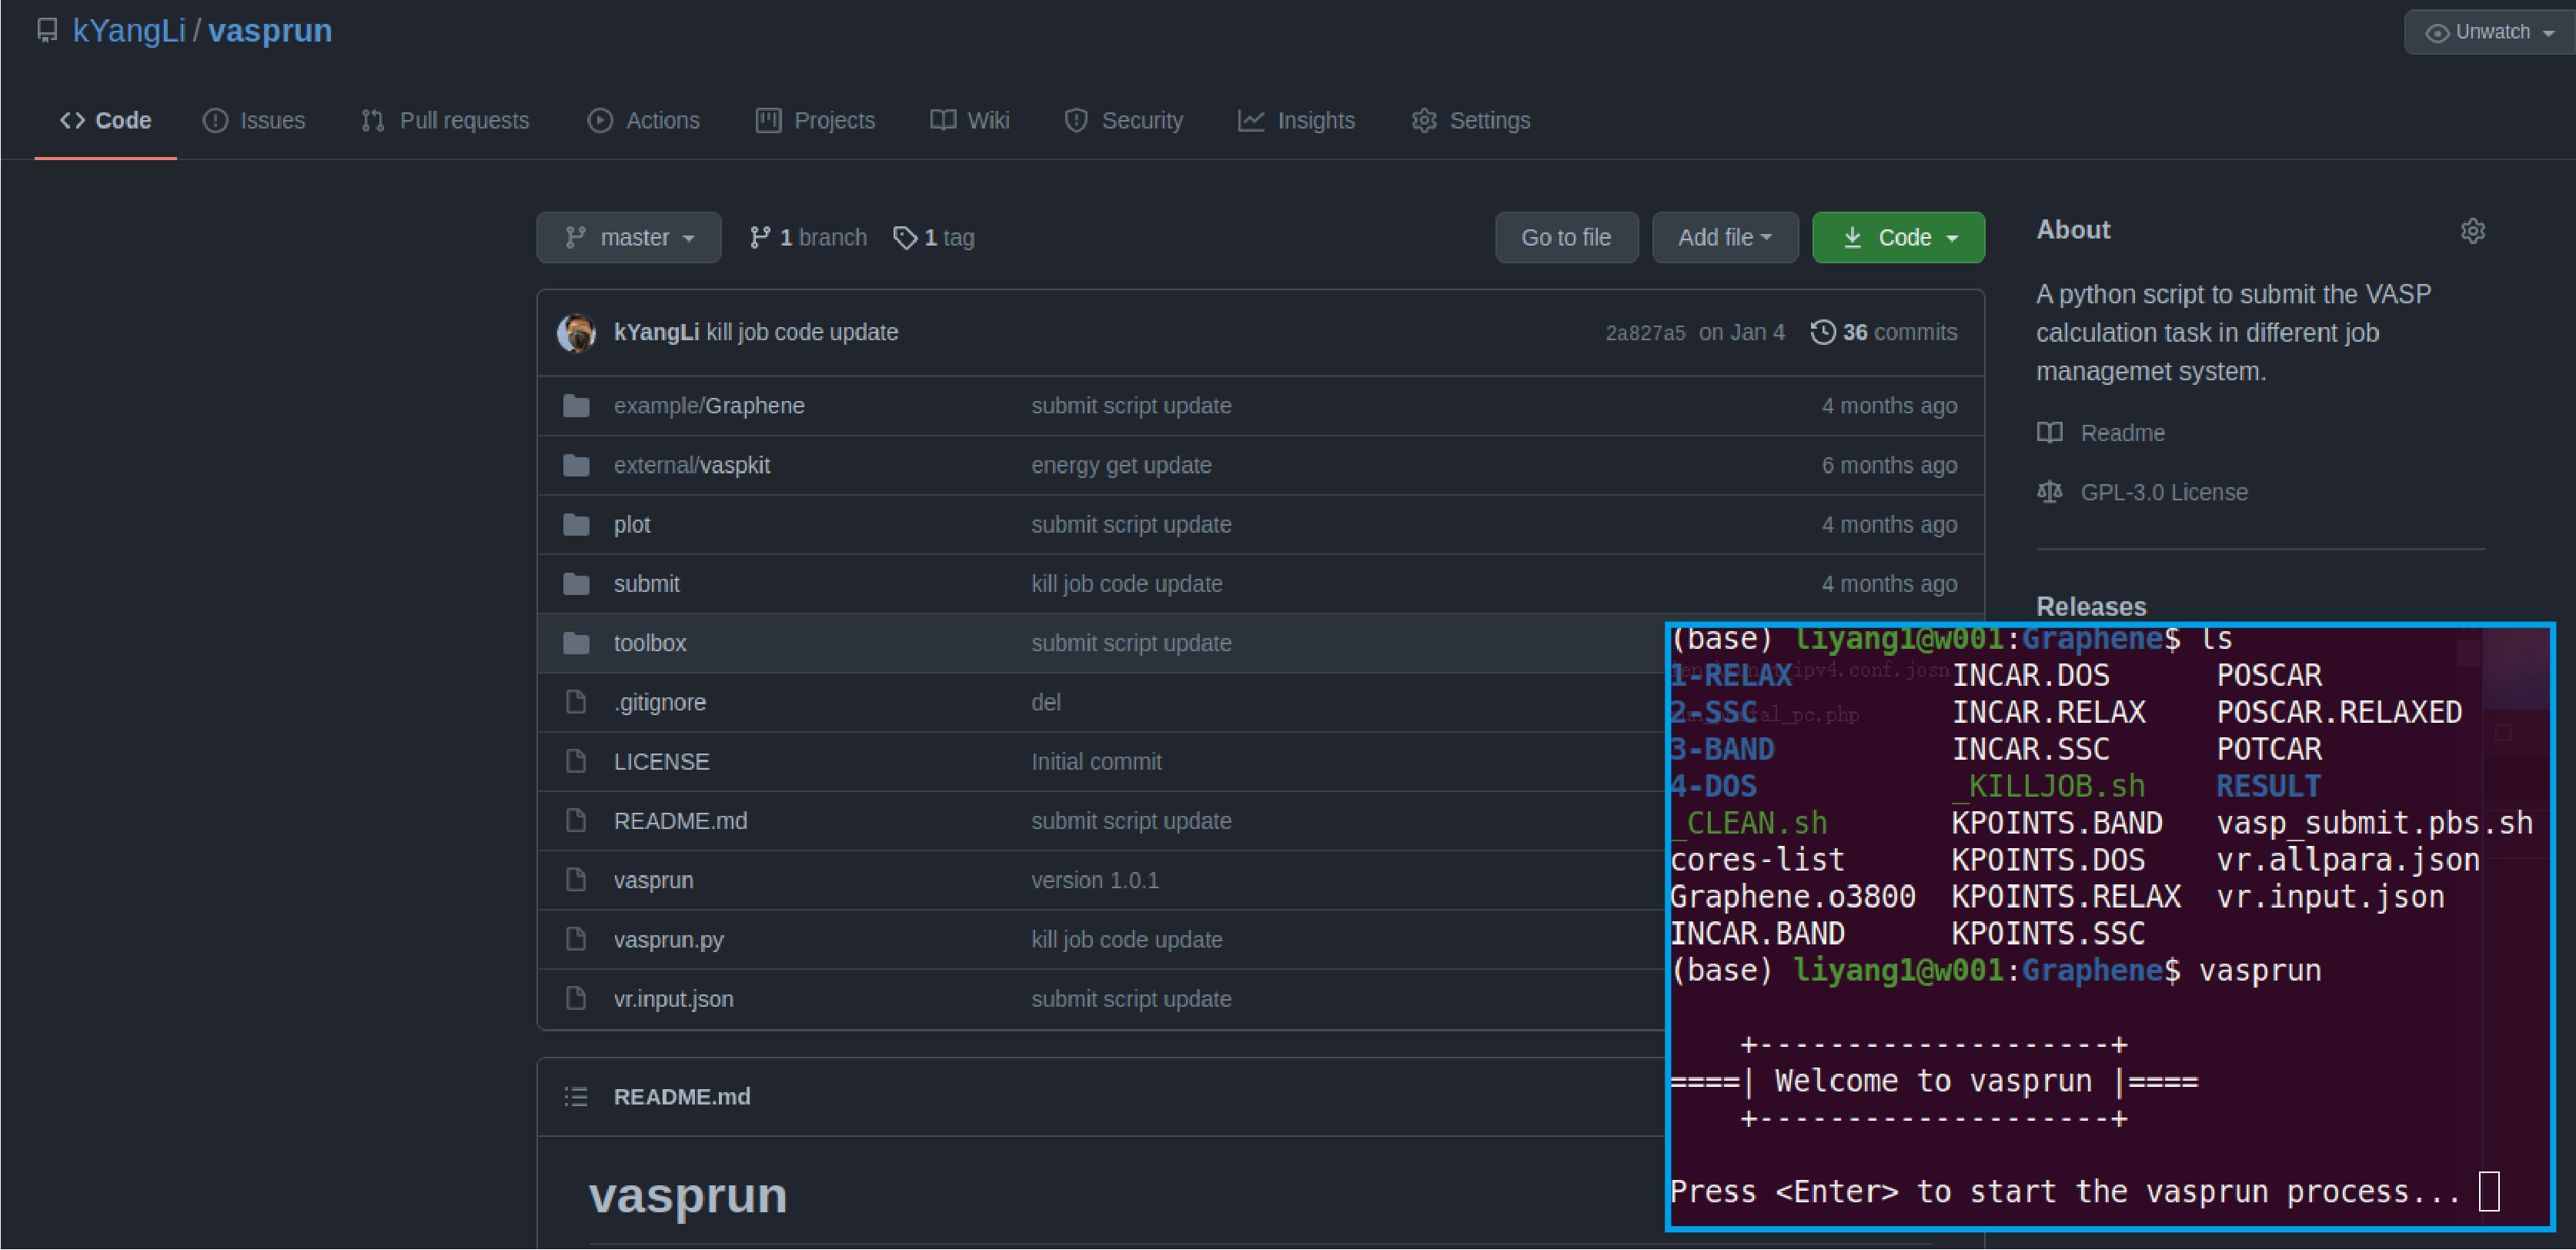
\includegraphics[width=\textwidth]{figure/vasprun.png}
      \end{tcolorbox}
    
      \begin{block}{}
        将计算任务写成流程化脚本, 可以极大的缩短在数据文件处理上的时间. 将重复劳动都交给计算机来做, 让我们有精力去思考更物理的问题.
      \end{block}
    \end{frame}
    %-===================================================================-%
  
    %+===================================================================+%
    \begin{frame}{编程应用4: 进行TB模型计算}
      \centering
      \begin{tcolorbox}[beamer,width=0.85\textwidth,arc=0pt,boxsep=0pt,left=0pt,right=0pt,top=0pt,bottom=0pt]
        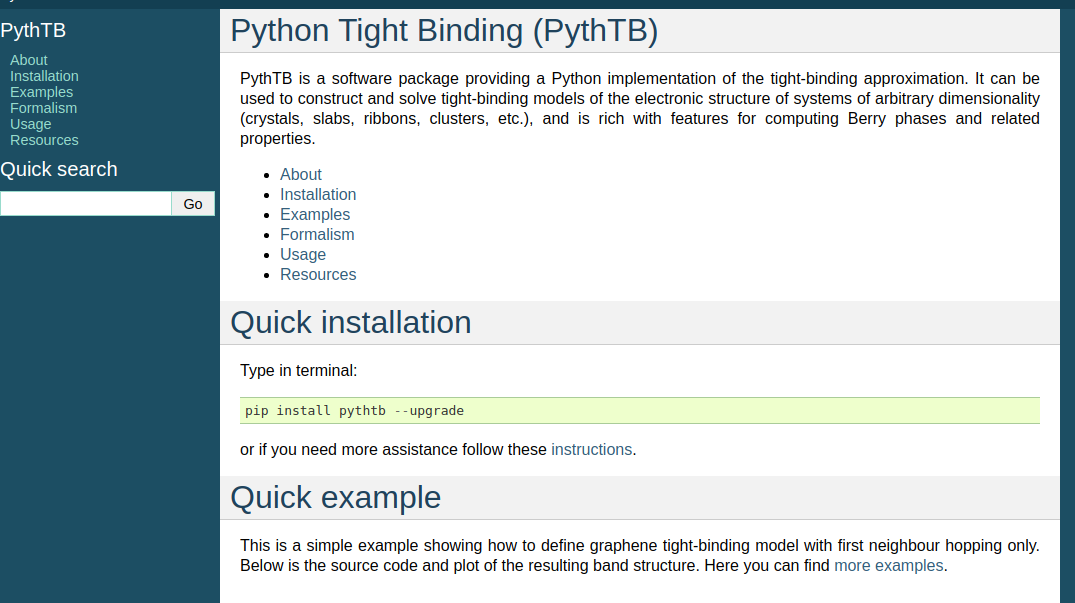
\includegraphics[width=\textwidth]{figure/ptb.png}
      \end{tcolorbox}
    
      \begin{block}{}
        使用别人造好的``轮子'', 站在前人的肩膀上, 才能更快更好地取得下一步进展. 科学的进步固然需要瞬间的灵感, 但更需要持久的积累. 而积累则是需要媒介的.
      \end{block}
    \end{frame}
    %-===================================================================-%

    %+===================================================================+%
    \begin{frame}{编程应用5: 机器学习与大数据}
      \centering
      \begin{tcolorbox}[beamer,width=0.8\textwidth,arc=0pt,boxsep=0pt,left=1pt,right=1pt,top=1pt,bottom=1pt]
        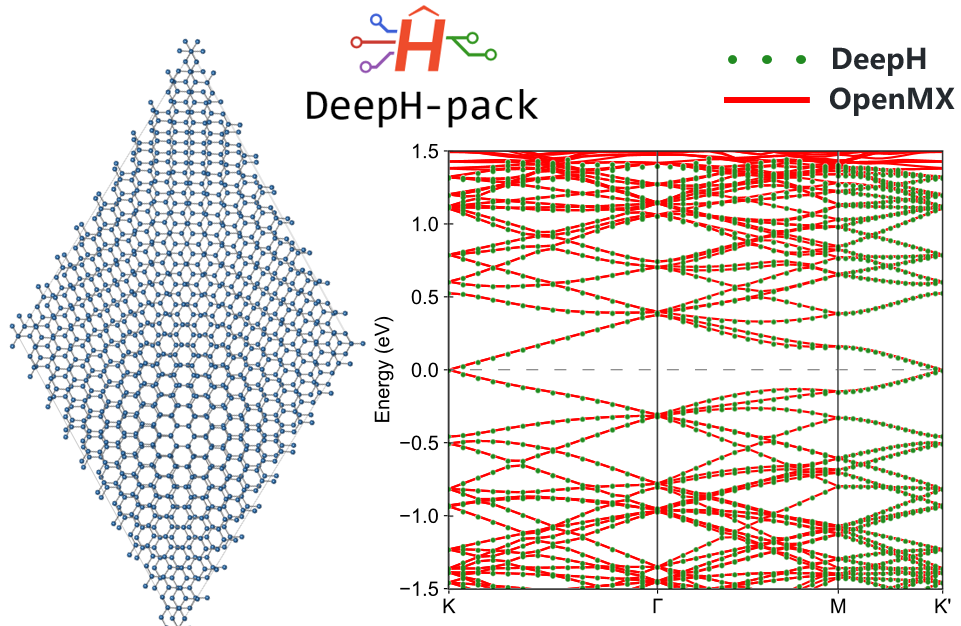
\includegraphics[width=\textwidth]{figure/deeph.png}
      \end{tcolorbox}
      \begin{block}{}
        自从计算机算力大幅提升后, 机器学习和大数据无疑成为了计算机领域最为火爆的项目.
      \end{block}
    \end{frame}
    %-===================================================================-%

    %+===================================================================+%
    \begin{frame}[fragile]{数据处理的基本内涵}
      \begin{block}{}
         一般来说, 数据处理无非就是依靠计算机完成以下三步: \purple{获取数据, 处理数据, 输出数据.}
         \begin{itemize}
           \item 数据源可能有多种来源, 例如, 存放在硬盘中, 由实验仪器串口通讯获得, 位于计算机内存中, 由人手动输入, 等. 下面我们将讨论大家最容易接触到的一类情况: 以文件的形式存放在硬盘中的数据处理. 
           \item 如何处理数据一般是跟具体的科研过程有关, 一般要做好这一步首先要非常明白: 自己有什么、自己要什么. 而后心思细密地函数式地逐步完成中间数据处理工作.
           \item 数据输出的方向也是多种多样的, 例如可以直接打印在屏幕上, 存储在硬盘文件中, 存储在内存中供下一级程序调用, 通过\cverb|UDP|或\cverb|TCP|协议通过网卡传送到另一台机器或CPU上进行协同处理, 或者输入回实验仪器使数据转换为具体的实验操作. 下面我们也将只讨论存储进硬盘这一种情况. 
         \end{itemize}
      \end{block}
      \purple{从硬盘某个文件读取数据, 处理他们, 并保存进新的文件.}
    \end{frame}
    %-===================================================================-%

  \section{学习编程前应具备的认识}
    %+===================================================================+%
    \begin{frame}{如何选择第一门语言}
      根据个人不同的需求, 可以选择不同的路径.
      \begin{block}{想系统地学习计算机编程}
        如果真的想非常系统的学习计算机编程知识, 在笔者看来, 应该首先学习计算机硬件知识. 了解计算机内部基本的组件和简要工作原理. 对计算机硬件系统有了大概了解之后, 学习的\purple{第一门高级语言}应该是离计算机底层较近的语言, 如C/C++. 而后在学会了函数式编程, 地址, 指针, 栈, 传参, 等概念之后, 可以开始着手学习用于快速开发且全平台适配性好的语言, 如Java 或 Python.
      \end{block}
      \begin{block}{想快速实现某个大规模数值计算或模拟程序 (如蒙卡)}
        一般需要选择一门静态语言进行学习. 如C/C++等.
      \end{block}
      \begin{block}{想快速做一下基于硬盘文件的数据处理}
        需要学习一个能快速开发并且便于和文件管理系统交互的语言, 如Python.
      \end{block}
    \end{frame}
    %-===================================================================-%

    %+===================================================================+%
    \begin{frame}{一个程序的基本组分}
      \begin{block}{个人对程序组分的解读}
        计算机程序其实就是一个复杂动作的实现流程, 这个流程一般由两部分组成, \textcolor{purple}{变量和算法}. 
      \begin{itemize}
        \item 变量是存储在计算机内存中的不同数据的代指, 每个变量都有一个变量名指定. 变量本身可以有不同的内部结构, 如浮点数, 整数, 字符串, 数组, 结构体等.
        \item 而算法则是操作这些变量相互作用的动作, 当然算法也可以更广义的理解为高度总结泛化后的程序流程. 算法靠顺序排列的流程控制语句和运算符实现.
        \item 一般来说, 一个程序所实现的复杂流程可以被拆分成不同子流程. 我们将这些子流程单独写出, 形成所谓的``函数'', 而后在主程序中通过函数调用将不同模块组合在一起, 完成指定动作. 因此也有人说, 程序的基本组分就是一个个\purple{``函数''}.
      \end{itemize}
    \end{block}
    \end{frame}
    %-===================================================================-%

    %+===================================================================+%
    \begin{frame}[fragile]{学会书写一个`好'程序}
      \begin{block}{编程时应尽量遵循的规则}
        \begin{itemize}\small
          \item 决定开始编写程序之前, 强烈建议您先大概浏览一下已有的编程规范, 例如``\href{https://zh-google-styleguide.readthedocs.io/en/latest/google-cpp-styleguide/}{\purple{谷歌编程规范}}'', 以防止学习过程中不良习惯的养成. 这些编程规范是在总结了海量的程序 Bug 出现情景后提出的. 遵循这些规范在让你的代码变得优雅易懂的同时, 也会极大地降低错误率.
          \item 一定要习惯并乐于书写\purple{注释}. 注释应该至少出现在那些你认为比较难懂不能一眼看出代码含义的地方. 别怕麻烦, 因为有了这些注释, 你的代码才能发扬广大. 俗话说的好, 己所不欲, 勿施于人, 即使你不认同这一点, 至少为了三个月后的自己着想一下. 而且, 合理的注释也能帮助您理清思路.
          \item \purple{变量命名}非常有讲究, 如果感觉使用\cverb|a|\cverb|b|\cverb|c|\cverb|i|\cverb|j|\cverb|k|\cverb|m|\cverb|n|\cverb|x|\cverb|y|式的变量命名非常自然, 那大概率您还没有经历过较大规模的程序开发.
          \item 如何界定一个\purple{函数}所管辖的范围是整个程序优雅性的精髓所在. 您的程序可不可以称为``好''程序, 很大一部分就取决于您如何界定和链接每个函数的功能.
          \item \purple{合理的换行}也是需要注意的. 没有人期望看到长达几百个字符的一行. 一般来说, 一行代码包括行首缩进不能超过80个字符.
        \end{itemize}
      \end{block}
    \end{frame}
    %-===================================================================-%

    %+===================================================================+%
    \begin{frame}{`好'程序内涵}
      \begin{block}{一句话定义什么是好程序}
        一个好的程序, 就是会让你在阅读这个程序时会由衷地感谢作者的贴心, 会不住地赞叹作者是真的在为读者着想.
      \end{block}
      程序写出来就是给人和机器看的. 机器比较死板, 如果它看不懂, 就会报错, 此时你就得到了一个无法正常运行的程序. 可以说, 让机器能看懂是一个程序的下限; 而让其他人能看懂, 则是一个优秀程序的下限.
    \end{frame}
    %-===================================================================-%

    %+===================================================================+%
    \begin{frame}[fragile]{如何书写注释}
      \begin{block}{}
        \begin{itemize}\small
          \item 注释不应该是复述某一步操作的表层意义是什么, 因为对于任何懂得这门语言的人, 都可以自发解读出来, 我们更应该用注释标明自己做此\purple{操作的动机}.
          \item 有人喜欢边写代码边注释, 有人喜欢写完代码后慢慢注释. 这都没有关系, 重要的是注释应当尽量在 ``你还记得此处详细思路, 并且不打断后续编程灵感''的条件下进行. 例如在你感觉需要放松一下或者要长舒一口气的时候, 可以写一写注释; 需要集中精神的时候, 可以用一个注释符标明这里应该有注释, 但现在没法停下来写他.
          \item 要善用\cverb|TODO|\purple{注释}. \cverb|TODO|标明了此处还需要继续开发, 但作者真的该回家陪老婆孩子了. 在你开始新的一天, 或从假期中返回时, 搜索一下\cverb|TODO|的位置就可以快速进入开发状态.
          \item 刚开始写注释, 你可能会非常不习惯. 有时可能会絮絮叨叨, 有时又会过于简略. 但没有关系, 多练几次, 慢慢习惯这种行为后, 你的语言会逐渐变得干练. 你将逐步学会如何清晰精准恰当地表述自己的意思.
        \end{itemize}
      \end{block}
    \end{frame}
    %-===================================================================-%

    %+===================================================================+%
    \begin{frame}[fragile]{如何命名变量}
      \begin{block}{}
        \begin{itemize}\small
          \item 变量名就是以下划线或字母开头的, 一堆字母数字下划线的组合. 如何在近乎无穷的组合中取到一个\purple{最优雅得体}的名字, 是非常值得学习的.
          \item 变量命名是一个非常需要讲究的东西. 应该时刻牢记, 我们取的每一个名字在未来会至少出现在某个师弟师妹的工作当中. 任何一个名字的形成, 经过了一段时间的混沌效应后, 都可能在未来诱导巨变. 变量名应该\purple{简洁明了地表达其本意}. 如果做不到简洁, 至少应该做到明了. 毕竟相较于代码的可读性, 程序文件是25K还是30K是不太重要的. 同时, 30个字符的变量名基本就是人类阅读舒适的极限.
          \item 如果你实在是喜欢 \cverb|a = b| 这种表述, 那至少也应该在这一行\purple{加入注释}, 解释一下 \cverb|a| \cverb|b| 分别代表什么.
          \item 如果你在写一个科学计算软件, 并已写好了相关的公式算法的Notes. 这时候, 在程序中不遵循编程规范中的约束, 并\purple{严格复用Notes中的符号}(如\cverb|S|, \cverb|x|, \cverb|H_ij|, \cverb|K_q|)是可取的, 前提是你可以确保看到这个程序的人同时一定可以看到你写的Notes. 在程序一开始声明``该程序中所有符号均与xx网址上的Notes相同"将是十分友善的做法.
        \end{itemize}
      \end{block}
    \end{frame}
    %-===================================================================-%

    %+===================================================================+%
    \begin{frame}[fragile]{如何定义函数}
      \begin{block}{}
        \begin{itemize}\small
          \item 函数的定义是非常非常值得注意的. 一个好的函数的定义是: \purple{该函数不能被继续拆分成若干子函数了}. 当然对于初学者来说, 要做到这一点非常困难. 因为对于我们这些不太熟悉编程的人来说, 光是想清楚该如何从程序层面上实现一整套操作就十分不容易了, 做到把问题拆解更是难上加难. 大多数时候都是走一步看一步. 但随着编程经历的增加, 我们会越来越体会到前人如此要求的良苦用心. 一个不良好定义的函数会让我们脑子一团浆糊, 并令人很容易就陷入到某些细枝末节的实现的愁苦情绪中, 失去对整个程序的把控.
          \item 同变量名一样, 函数名也应该\purple{言简意赅}地描述该函数的作用, 如 \cverb|get_magnetic_J()| 就是一个不错的名字, 他告诉读者, 这个函数的作用就是得到磁性交换相互作用系数J. 而 \cverb|gmj()| 就相对拉垮一些.
          \item 每个函数都应该有\purple{详细描述该函数功能的注释}. 注释应至少包括对该函数实现的功能的描述, 最好有对输入输出项的简要解释. 注意注释不应该以函数为第一人称, 而应该在第三人称视角描述函数作用.
          \item \purple{充分细化的函数}不但不会让程序复杂, 恰恰相反, 他会让程序看起来分外清爽.
        \end{itemize}
      \end{block}
    \end{frame}
    %-===================================================================-%

    %+===================================================================+%
    \begin{frame}[fragile]{定义函数示例}
      \begin{columns}
        \begin{column}{0.4\textwidth}
          \begin{block}{\tiny 良好定义的函数们}
            \begin{lstlisting}
def 举起(身体部位):
  pass #TODO   

def 展开(身体部位):
  pass #TODO 

def 对准(身体部位, 物体):
  pass #TODO 

def 缩紧(身体部位):
  pass #TODO 

def 拉回(身体部位):
  pass #TODO 

def 握住(手, 物体):
  展开(手)
  对准(手, 物体)
  缩紧(手)

def 摘(手, 物体):
  举起(手)
  握住(手, 物体)
  拉回(手)

def main():
  摘(手, 苹果)
            \end{lstlisting}
          \end{block}
        \end{column}
        \begin{column}{0.4\textwidth}
          \begin{block}{\tiny 不良好定义的函数们}
            \begin{lstlisting}
def 对准苹果(手):
  """这里实现了对准苹果的操作"""
  ...<一堆非常冗长的操作>

def bulibula():
  """实现了拿住苹果的操作"""
  ...<一堆操作>

def 摘苹果():
  # 下面实现了举起手的操作
  ...<一堆非常冗长的操作>
  # 下面实现了展开手的操作
  ...<一堆非常冗长的操作>
  对准苹果(手)
  bulibula()
  # 下面实现了拉回苹果的操作
  ...<一堆非常冗长的操作>

def main():
  摘苹果()
            \end{lstlisting}
          \end{block}
          \begin{block}{\tiny 什么是``好''函数}\tiny
            该函数不能被继续拆分成任何子函数. 
          \end{block}
        \end{column}
      \end{columns}
    \end{frame}
    %-===================================================================-%

    %+===================================================================+%
    \begin{frame}{规则不是障碍而是高效的保障}
      \begin{block}{过犹不及}
        \begin{itemize}
          \item 以上种种规范, 都是基于方便编程者和读者的角度提出的. 无论对于程序开发者还是阅读者, 他们无疑都是非常善意的提醒. 但作为初学者的我们也不要被这些条条框框约束地不敢写代码, 一步三回头. 须知, \purple{大胆尝试, 小心验证}. 只有代码水准到了更高的层次才能更好的践行这些准则.
          \item 遇到错误第一时间想到的应该是\purple{先看报错信息}, 分析无果后可以上网查证, 也可以数值验证. 具体该如何Debug我们会在稍后Slides中说明.
        \end{itemize}
      \end{block}
    \end{frame}
    %-===================================================================-%

    %+===================================================================+%
    \begin{frame}{什么是面向对象的编程?}
      \begin{block}{定义}
        \purple{面向对象区别于面向过程}\textcolor{gray}{(面向过程就是按照问题描述, 按部就班地完成一系列操作. 面向过程的核心是``过程''如何一步步实现)}, 在解决问题时, 它会\purple{把``过程''中出现的事物抽象成对象(Object)}, 然后给予对象一些属性和方法. 而后通过对象间属性、方法的相互作用实现程序目标.
      \end{block}
      \begin{block}{特性}
        \begin{itemize}
          \item 相较于面向过程, 面向对象\purple{更贴近人类思考事物的思维模式}. 因此在面对一些复杂功能时, 面向对象往往更轻松就能实现.
          \item 面向对象有三大特点: \purple{封装, 继承, 多态}.
          \item 面向对象编写的程序, 性能一般比面向过程低. 但其易维护、易复用、易扩展, 代码不同模块间耦合度很低, 整个代码系统灵活有序.
          \item 科学计算一般使用面向过程编程, 复杂过程一般使用面向对象编程.
          \item 从面向过程到面向对象, 类似于, 从牛顿力学到理论力学.
        \end{itemize}
      \end{block}
    \end{frame}
    %-===================================================================-%

    %+===================================================================+%
    \begin{frame}[fragile]{面向对象代码示例}
      \begin{columns}
        \begin{column}{0.4\textwidth}
          \begin{block}{\tiny 面向过程编程}
            \begin{lstlisting}
def 举起(身体部位):
  pass #TODO   

def 展开(身体部位):
  pass #TODO 

def 对准(身体部位, 物体):
  pass #TODO 

def 缩紧(身体部位):
  pass #TODO 

def 拉回(身体部位):
  pass #TODO 

def 握住(手, 物体):
  展开(手)
  对准(手, 物体)
  缩紧(手)

def 摘(手, 物体):
  举起(手)
  握住(手, 物体)
  拉回(手)

def main():
  摘(手, 苹果)
            \end{lstlisting}
          \end{block}
        \end{column}
        \begin{column}{0.4\textwidth}
          \begin{block}{\tiny 面向对象编程}
            \begin{lstlisting}
class 身体部位():
  def __init__(self):
    pass # Nothing done
  def 举起(self):
    ...<实现了身体部位的举起>
  def 展开(self):
    ...<实现了身体部位的展开>
  def 缩紧(self):
    ...<实现了身体部位的缩紧>
  def 对准(self, 物体):
    ...<实现了身体部位对准某物体>
  def 拉回(self):
    ...<实现了身体部位的拉回>

class 手(身体部位):
  def 握住(self, 物体):
    self.展开(手)
    self.对准(手, 物体)
    self.缩紧(手)
  def 摘(self, 物体):
    self.举起(手)
    self.握住(手, 物体)
    self.拉回(手)
  
def main():
  我的手 = 手()
  我的手.摘(苹果)
            \end{lstlisting}
          \end{block}
        \end{column}
      \end{columns}
    \end{frame}
    %-===================================================================-%

    %+===================================================================+%
    \begin{frame}{游戏中的面向对象编程}
      \begin{center}
        \begin{tcolorbox}[beamer,width=0.8\textwidth,arc=0pt,boxsep=0pt,left=0pt,right=0pt,top=0pt,bottom=0pt]
          
\includegraphics[width=\textwidth]{figure/zad.png}
        \end{tcolorbox}
      \end{center}
      \begin{block}{\small 设想编程实现如下功能}\small
        下雨\purple{天}时, \purple{人物}躲在\purple{树}荫下, 此时一道\purple{闪电}劈过来, 人物手中的\purple{火把}连同树荫下的\purple{草地}都被闪电点燃. 人物走出树荫, 火把又被雨\purple{水}浇灭.
      \end{block}
    \end{frame}
    %-===================================================================-%

    %+===================================================================+%
    \begin{frame}{如何学习一门编程语言}
      如同绝大部分语言一样, 学会并熟练掌握一门编程语言的最有效方法就是多看多练. 学习编程时, 一定要保证自己是可以访问互联网的.
      \begin{block}{以笔者个人Python学习为例}
        \begin{itemize}
          \item 首先笔者去``菜鸟教程''系统地学习关于python的所有基础内容. 
          \item 而后花了两周时间, 第一周先尝试编写一些小程序, 如识别回文数, 产生斐波那契数列, 解一元二次方程组, 寻找1E10以下的质数, 等. 
          \item 而后在后面一周, 通过python尝试编写出了一个\href{https://github.com/kYangLi/Game-Skyround}{\purple{地牢探险游戏}}. 那两周就是一直在上网查``python中如何实现xxx'' ``python错误xxx'', 然后不断尝试网页上的提示, 不断与各种bug斗智斗勇, 在此过程中对python的理解也加深了不少, 也乐在其中.
          \item 接着, 等到笔者认为自己基本理解了python的使用之后, 又去``菜鸟教程''浏览了一遍其内容. 查缺补漏.
          \item 之后就是不断将自己学到的python编程知识应用到实践中, 不断认识、否定认识、再认识. 直到现在也在一直学习.
        \end{itemize}
      \end{block}
    \end{frame}
    %-===================================================================-%

  \section{学习Python前的准备工作}
    %+===================================================================+%
    \begin{frame}[fragile]{正确安装Python (Conda)}
      \begin{center}
        \begin{tcolorbox}[beamer,width=0.76\textwidth,arc=0pt,boxsep=0pt,left=0pt,right=0pt,top=0pt,bottom=0pt]
          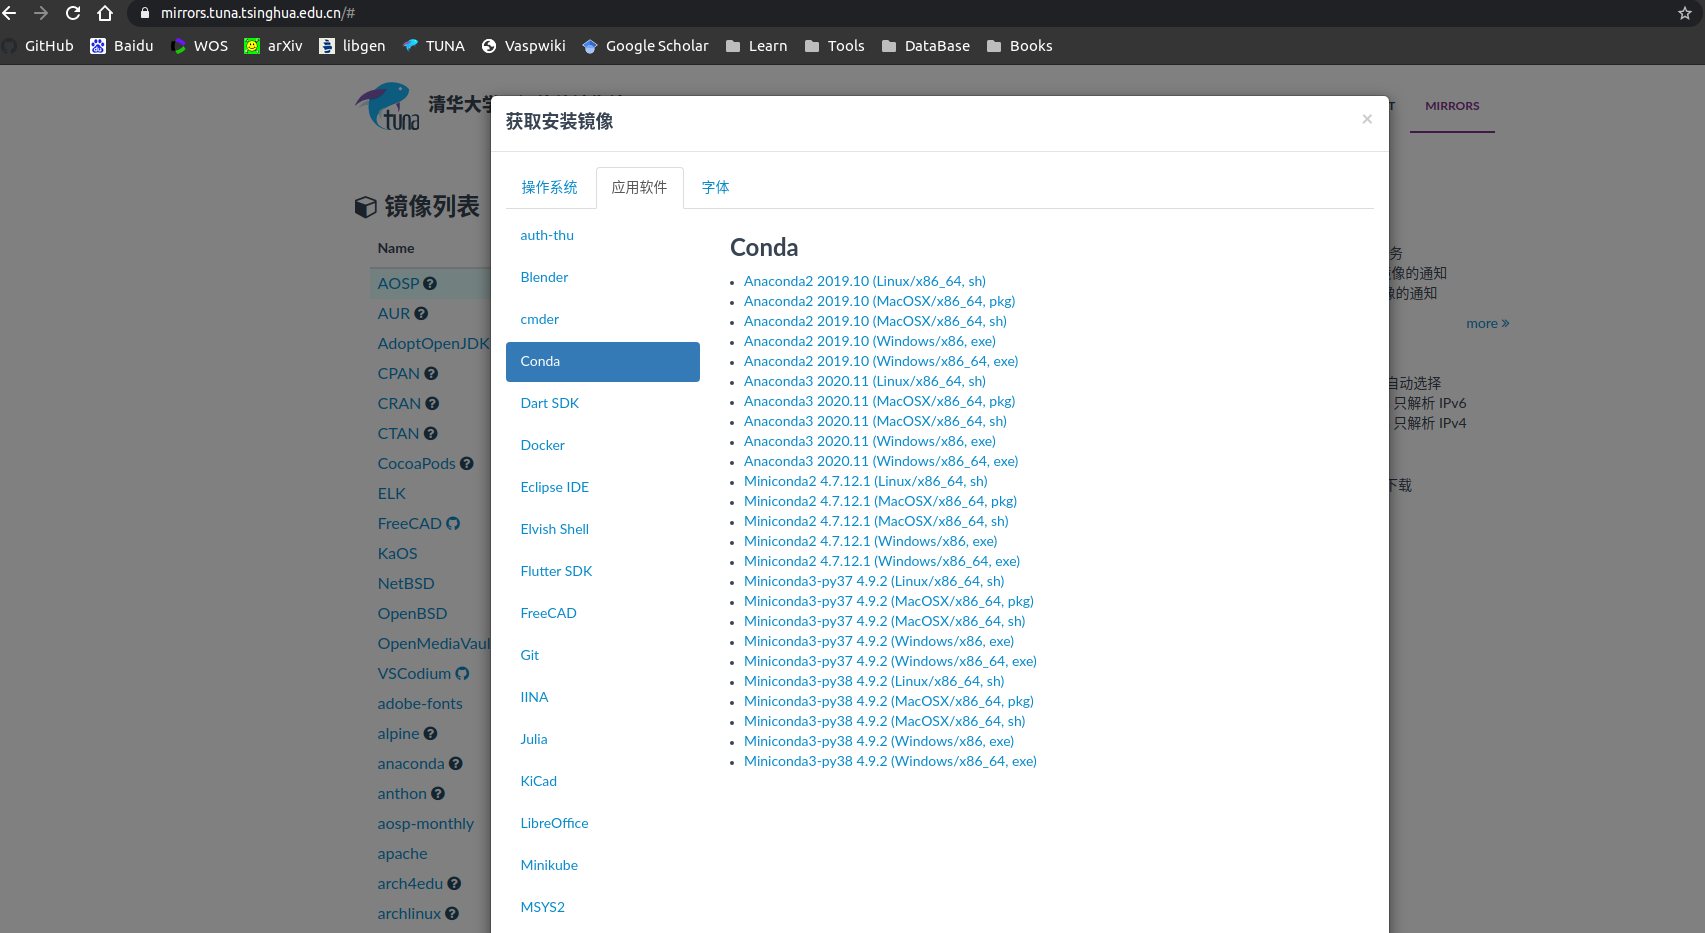
\includegraphics[width=\textwidth]{figure/conda.png}
        \end{tcolorbox}
      \end{center}
      \begin{block}{\small 安装Anaconda3}\small 
        前往\href{https://mirrors.tuna.tsinghua.edu.cn/}{\purple{清华镜像站}}, 点击右侧边栏中的``获取下载链接'', 获取最新版Anaconda3下载包. \cverb|conda|是python的包管理器. 此软件可以高效便捷地管理python环境. 可访问其\href{https://docs.conda.io/projects/conda/en/latest/user-guide/getting-started.html}{\purple{帮助文档}}, 学习如何使用\cverb|conda|指令. 在python代码开发时, 使用环境管理器是至关重要的, 它可以省去很多麻烦.
      \end{block}
    \end{frame}
    %-===================================================================-%

    %+===================================================================+%
    \begin{frame}{高效使用编辑器或IDE}
      \begin{block}{工欲善其事, 必先利其器.}
        能高效的使用一款编辑器或者python IDE是非常关键的. 笔者曾见过有人使用word写代码, 当时心中五味杂陈, 也不免对其编写的程序多了几分忌惮. \textcolor{gray}{就好像是走在大街上迎面遇到了几个红绿头发说着火星文的花里胡哨的年轻男子.}

        言归正传, 能正确使用一款高效的编辑器/IDE, 才能最大限度地提升码代码的舒适度和效率, 也能在一定程度上提高Debug的精准度. 高的编程效率和低的错误率总是我们所期望的.
        
        如果让笔者推荐一款编辑器, 我大概会推荐由微软推出的 \href{https://code.visualstudio.com}{\purple{VS Code}}. 如果说推荐一款IDE, 笔者就没有什么经验了, 但好像大家都在用 \href{https://www.spyder-ide.org}{\purple{Spyder}}. 
      \end{block}
    \end{frame}
    %-===================================================================-%

    %+===================================================================+%
    \begin{frame}{提升工作环境}
      \begin{block}{工欲善其事, 必先利其器.} 
        \begin{itemize}
          \item 如果您希望能开始专业写代码工作, 那么一个舒适高效的工作环境是必不可少的. 试想, 用一块手机屏幕学编程, 和同时用两块屏幕, 一块写代码, 一块看教程看结果. 其效率显然是不同的. 
          \item 因此作为初学者, 笔者建议至少配备一台笔记本, 或者一个带显示屏的主机, 之后根据个人工作需求添加额外配置即可. 同时要保证, 您的机器是可以访问网络的.
          \item 另外, 根据笔者的经验, 竖屏对编程和浏览文献是更加友好的; 将Linux作为生产主机会比Windows高效一些.
          \item 同时要杜绝消费主义, 我们的配套设施满足需求即可, 不必追求过于奢华的配置.
        \end{itemize}    
      \end{block}
    \end{frame}
    %-===================================================================-%

    %+===================================================================+%
    \begin{frame}{笔者的工作环境}
      \begin{center}
        \begin{tcolorbox}[beamer,width=0.8\textwidth,arc=0pt,boxsep=0pt,left=0pt,right=0pt,top=0pt,bottom=0pt]
          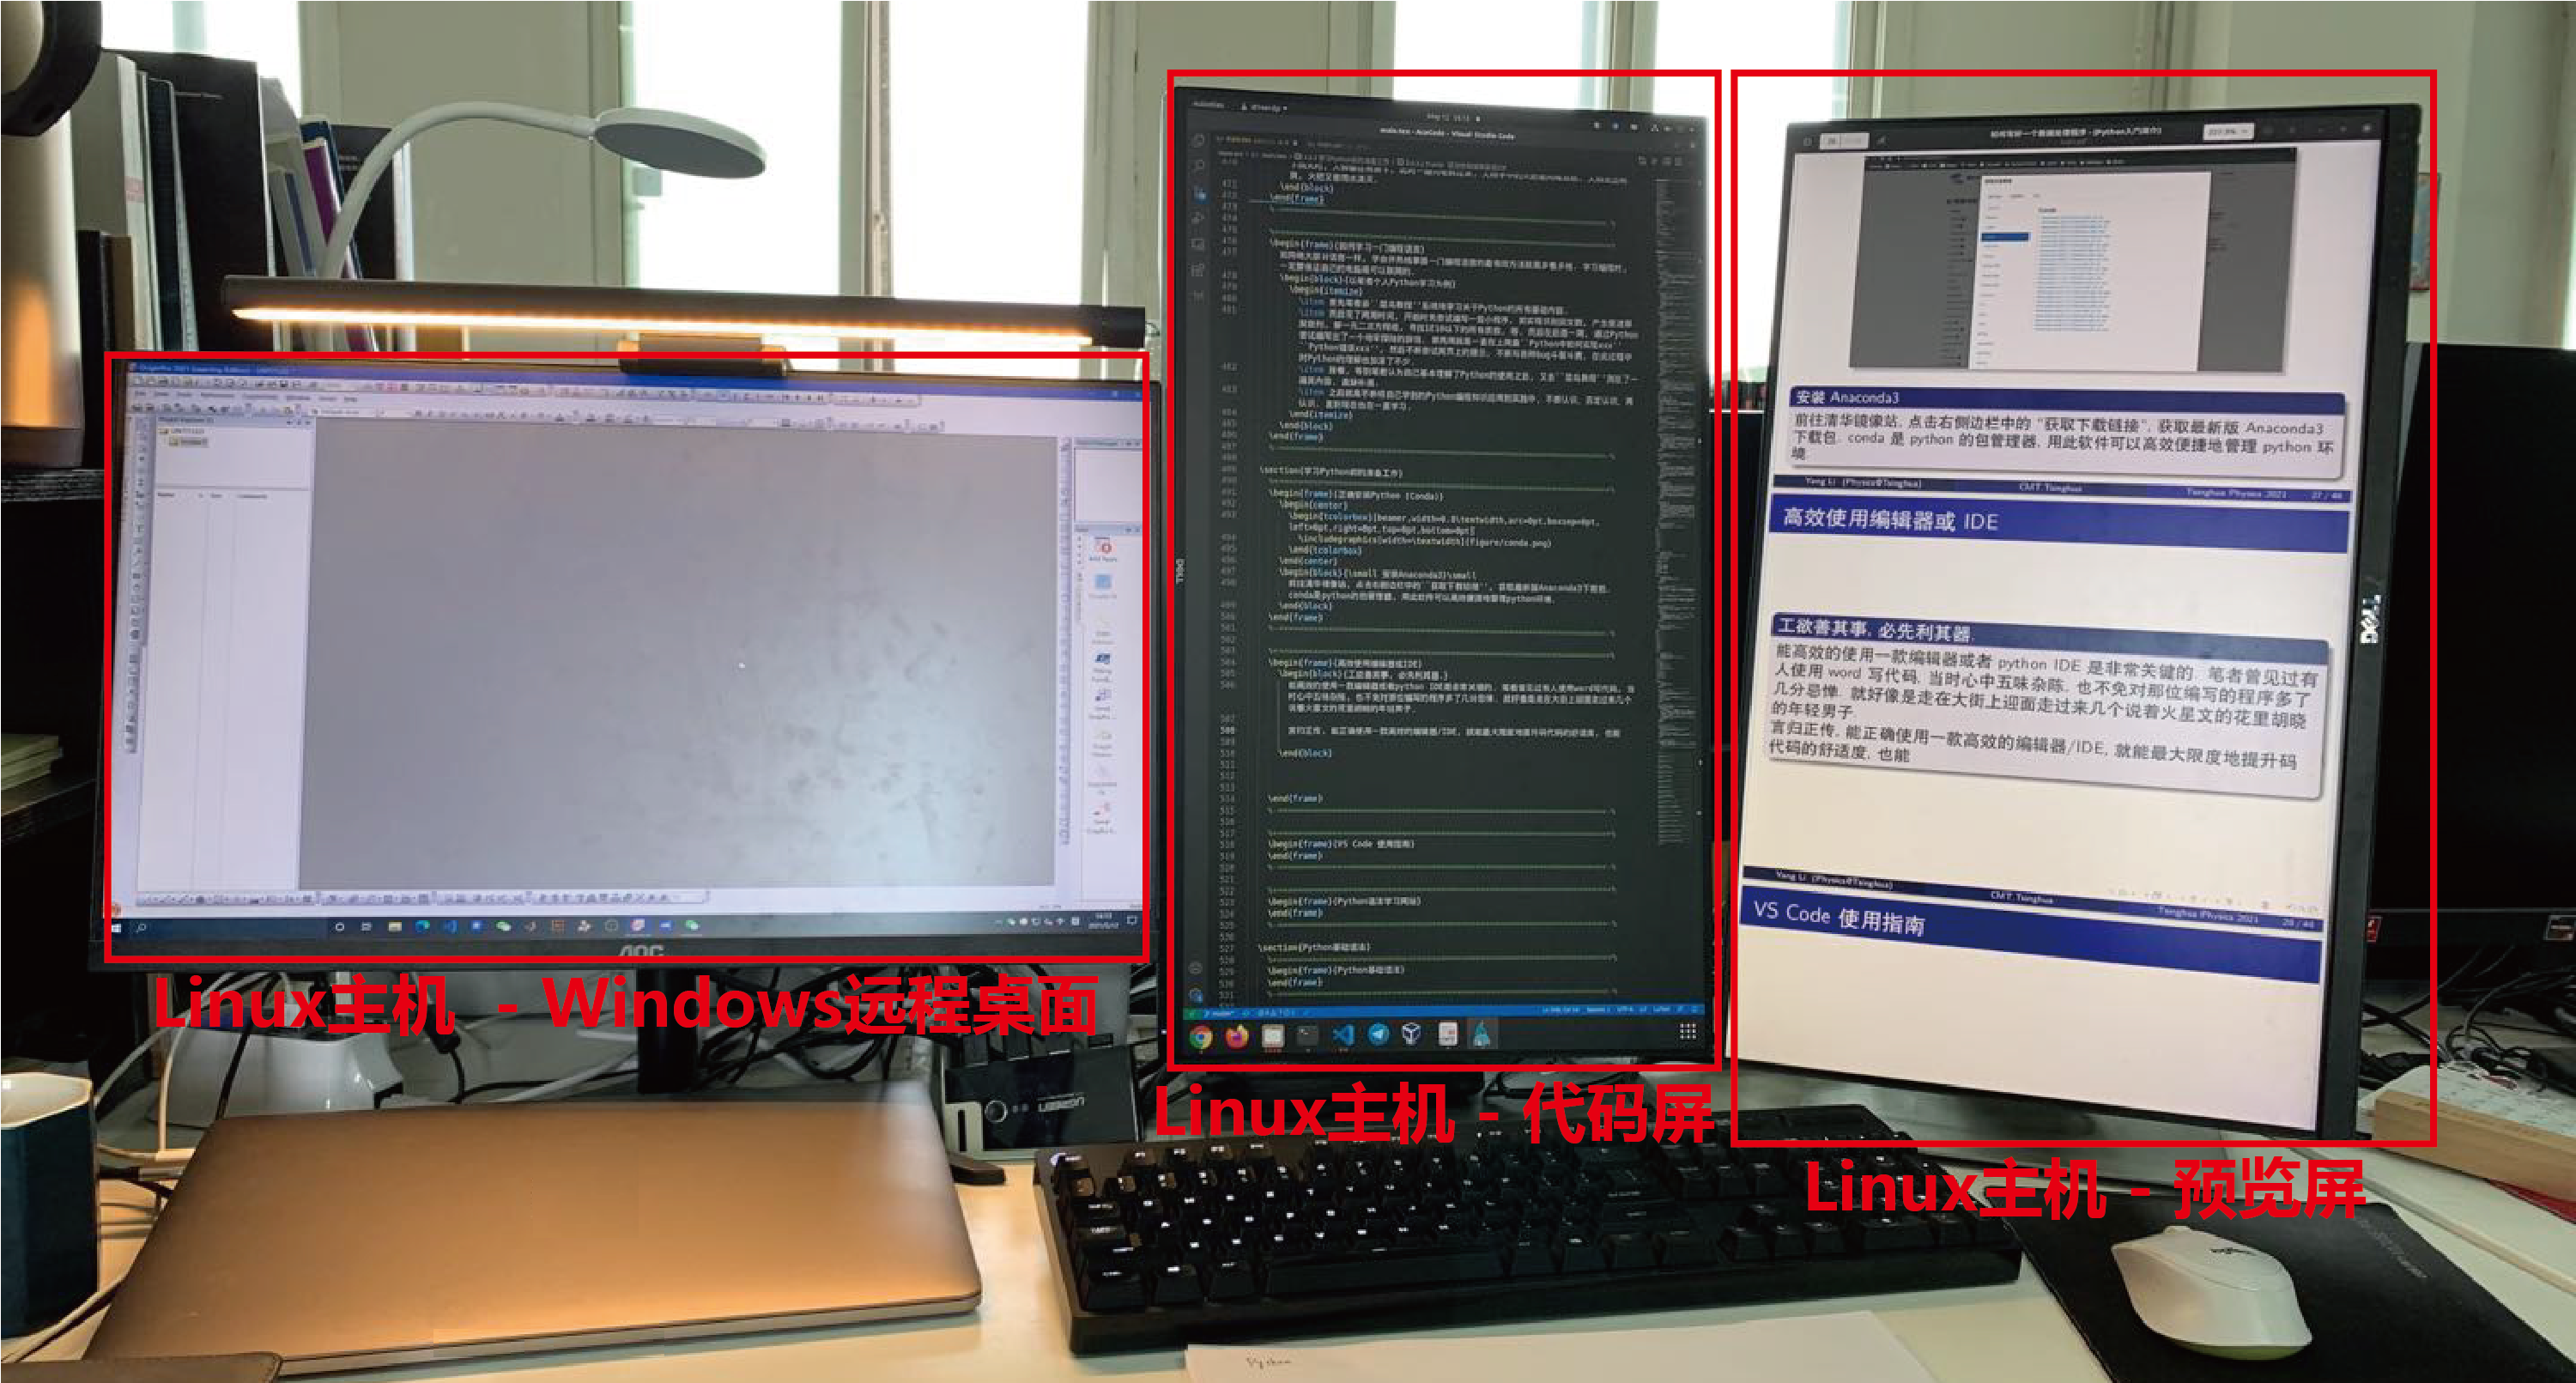
\includegraphics[width=\textwidth]{figure/env.png}
        \end{tcolorbox}
      \end{center}
      \begin{block}{\scriptsize 目前的工作环境}\scriptsize
        \begin{itemize}
          \item 一台装载\purple{Ubuntu系统}、配置中游、与三块屏幕相连的主机, 作为\purple{主要生产工具}. 主要用于代码开发、文献调研、数据分析、\LaTeX 文档书写、三维图片渲染等工作.
          \item 一台装载\purple{Windows系统}、配置下游、通过远程桌面访问的主机, 作为\purple{辅助生产工具}. 主要用于 Origin精修数据图、Office全家桶文档书写、微信交流等.
        \end{itemize}
      \end{block}
    \end{frame}
    %-===================================================================-%

    %+===================================================================+%
    \begin{frame}[fragile]{VS Code 使用指南}
      \begin{block}{}
        \begin{itemize}
          \item  毫不夸张地说, 自VS Code出现之后, 他基本碾压了其他所有的\purple{编辑器}. 现在的\cverb|VS Code|就如同当年的\cverb|vim|和\cverb|emacs|一样风靡. 
          \item  VS Code 的火热很大程度上是因为其优雅的外观和丰富的插件.
          \item  VS Code 给广大开发者提供了插件开发的接口. 并由此诞生了数目众多的外接扩展库, 如\cverb|C/C++|, \cverb|LaTeX Workshop|, \cverb|Remote-SSH|, \cverb|Python|, \cverb|Jupyter|, \cverb|Prettier|等等. 这些扩展库有些是广受欢迎的, 拥有千万级的订阅量. 例如 \cverb|LaTeX Workshop| 插件的\LaTeX 保存即编译功能就会让你爱不释手. 已被python官方插件 \cverb|Python| 吸收 \cverb|Pylance| 插件, 会让代码看起来非常舒适, 也极大地降低了语法错误率. 
        \end{itemize}
      \end{block}
      \begin{block}{}
        让我们简单演示几个Python在VS Code中使用的例子.
      \end{block}
    \end{frame}
    %-===================================================================-%

    %+===================================================================+%
    \begin{frame}{Python语法学习网站}
      计算机语言学习不同于其他知识, 他在互联网上的分布非常广泛, 只要你愿意, 在搜索引擎中输入`Python教程', `python tutorial'等关键字, 就可以搜索出众多高质量的教程.
      \begin{block}{}
      
        \begin{center}
          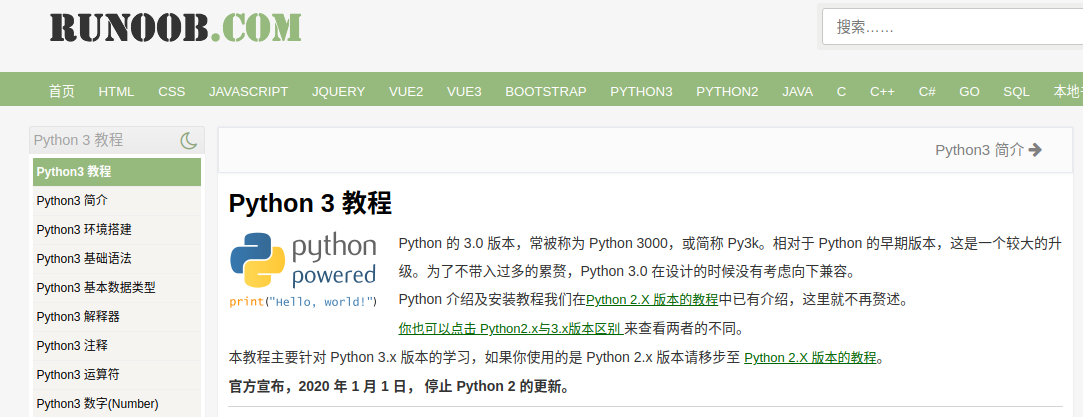
\includegraphics[width=\textwidth]{figure/noob.png}
          % \begin{tcolorbox}[beamer,width=\textwidth,arc=0pt,boxsep=0pt,left=0pt,right=0pt,top=0pt,bottom=0pt]
          %   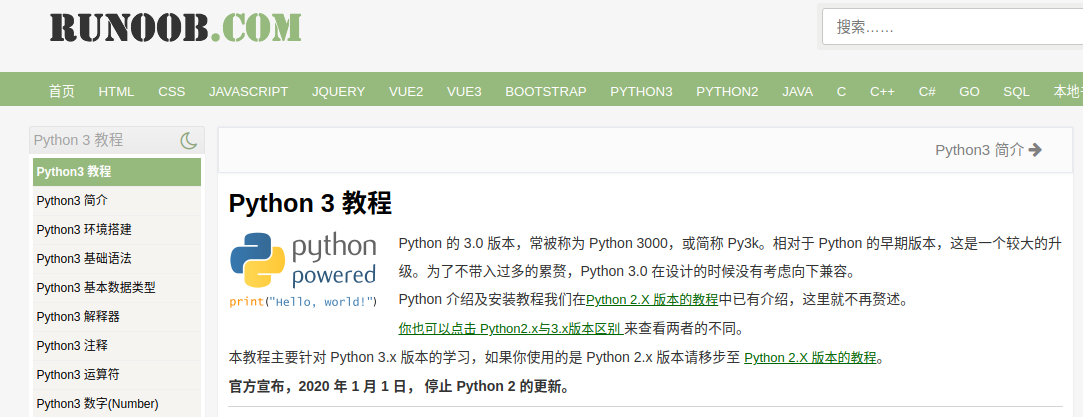
\includegraphics[width=\textwidth]{figure/noob.png}
          % \end{tcolorbox}
          \centering\purple{\small\url{https://www.runoob.com/python3/python3-tutorial.html}}
        \end{center}
      \end{block}
    \end{frame}
    %-===================================================================-%

  \section{Python基础语法}
    %+===================================================================+%
    \begin{frame}[fragile]{Python基础语法}
      \begin{block}{}
        \begin{itemize}
          \item Python 对大小写敏感, 所有名称或标志符必须以字母或下划线开头, 并由字母、数字、下划线构成.
          \item Python 中单行注释以井号 \cverb|#| 开头. 可以使用三引号\cverb|"""..."""| \cverb|'''...'''| 对应的字符串块进行多行注释.
          \item 与大多数语言不同, python不依靠首末起止符(如左右大括号 \cverb|{...}|)标定代码块, 而是通过行首缩进格数区分代码结构. 这就引出了 python 编程规范里一条非常重要的要求: 在任何时候都不要使用 \cverb|TAB| 键自动缩进.
          \item 如果感觉一行写不开, 可以用反斜线\cverb|\| 来实现代码换行. 同时某些位置(例如被圆括号括\cverb|(...)|起来的两行)的换行是不需要反斜线标定的.
          \item 使用\cverb|print()|函数可以将目标参数输出至标准输出(终端显示屏).
          \item Python是解释型语言. 也即他的代码是逐行单独运行的.
        \end{itemize}
      \end{block}
      \textcolor{gray}{\small 请注意, 由于PDF编码问题, 请勿复制本Slides中的任何符号或代码到程序中.}
    \end{frame}
    %-===================================================================-%

    %+===================================================================+%
    \begin{frame}[fragile]{变量类型和运算符}
      \begin{block}{\footnotesize 变量}
        \begin{itemize}\footnotesize
          \item True, False, None
          \item 整数, 浮点数
          \item 字符串
          \item 列表, 元组, 字典, 集合
        \end{itemize}
      \end{block}

      \begin{block}{\footnotesize 运算符}
        \begin{table}\scriptsize
          \begin{tabular}{r|l}
            \toprule
            \cverb|+| \cverb|-| \cverb|*| \cverb|/| & 加, 减, 乘, 除\\
            \midrule
            \cverb|//| \cverb|%| \cverb|**| & 整除(向下取整), 模, 幂  \\
            \midrule
            \cverb|==| \cverb|!=| \cverb|>| \cverb|>=| \cverb|<| \cverb|<=| & 逻辑等于, 不等于, 大于, 大于等于, 小于, 小于等于\\
            \midrule
            \cverb|=| & 赋值等于\\
            \midrule
            \cverb|+=| \cverb|-=| \cverb|*=| \cverb|/=| \cverb|//=| \cverb|%=| \cverb|**=|  & 赋值加等, 减等, 乘等, 除等, 整除等, 模等, 幂等\\
            \midrule
            \cverb|&| \cverb!|! \cverb|~| \cverb|^| \cverb|<<| \cverb|>>| & 按位与, 或, 非, 异或, 左移, 右移\\
            \midrule
            \cverb|and| \cverb|or| \cverb|not| \cverb|in|      &并且, 或者, 不是, 包含\\
            \bottomrule
          \end{tabular}
        \end{table}
        \end{block}
    \end{frame}
    %-===================================================================-%

    %+===================================================================+%
    \begin{frame}[fragile]{流程控制语句}
      \begin{block}{概述}
        \begin{itemize}\small
          \item \cverb|if| \cverb|(condition):| ... \cverb|elif| ... \cverb|else| ...
          \item \cverb|for| \cverb|(condition):| ...
          \item \cverb|while| \cverb|(condition):| ...
          \item \cverb|break|, \cverb|continue|, \cverb|pass|
        \end{itemize}
      \end{block}
      \begin{exampleblock}{if 判断}
        \begin{lstlisting}
if iamyourfather(me.name):
  me.get_money(1E9)
else:
  print("No, I believe in Yoda.")
        \end{lstlisting}
      \end{exampleblock}
      \begin{exampleblock}{for 循环}
        \begin{lstlisting}
for index in range(10):
  print('Yoo! %d' %(index,))
print("I finally find you!")
        \end{lstlisting}
      \end{exampleblock}
    \end{frame}
    %-===================================================================-%

    %+===================================================================+%
    \begin{frame}[fragile]{函数声明与定义}
      \begin{center}
        \begin{tcolorbox}[beamer,width=0.7\textwidth,arc=0pt,boxsep=0pt,left=1pt,right=1pt,top=1pt,bottom=1pt]
          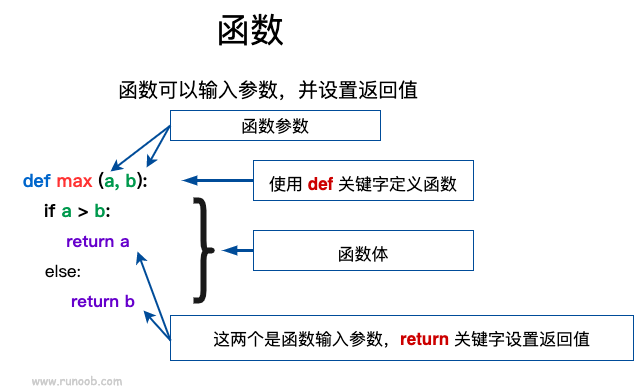
\includegraphics[width=\textwidth]{figure/defhs.png}
        \end{tcolorbox}\\
        \textcolor{gray}{\tiny Cite from www.runoob.com}
      \end{center}
      \begin{exampleblock}{}
        \begin{lstlisting}
def iamyourfather(a_name):
  if a_name == 'father':
    return True
  return False 
        \end{lstlisting}
      \end{exampleblock}
    \end{frame}
    %-===================================================================-%
    %+===================================================================+%
    \begin{frame}[fragile]{如何安装和导入一个外部模块}
      \begin{block}{安装}
        您可以使用 \cverb|conda install [pkg]| 指令安装指定包.\\ 
        {\tiny 您可能也听说过可以使用\cverb|pip| 来安装python包. 但随着对python使用的深入, 您会越来越体会到\cverb|conda|环境管理器的便捷之处.}
      \end{block}
      \begin{block}{导入}
        使用\cverb|import|指令导入被安装好的模块.
        \begin{lstlisting}
import os
import numpy as np
import matplotlib.pyplot as plt
from scipy import optimize
from math import *
        \end{lstlisting}
      \end{block}
      \begin{block}{导入规范}
        \begin{itemize}
          \item 一般\cverb|import|语句仅会出现在文件最开头.
          \item 单个\cverb|import|中不建议导入多个库的内容.
          \item 某些库的导入是有建议顺序的.
        \end{itemize}
      \end{block}
    \end{frame}
    %-===================================================================-%
    %+===================================================================+%
    \begin{frame}[fragile]{面向对象编程}
      \begin{block}{}\small
        构造对象包括构建对象的属性和方法. 对象的属性就是在对象所对应的类中定义的变量, 对象的方法就是类中定义的函数.
        \begin{lstlisting}
class ClassName():
  ...<some_statement>
        \end{lstlisting}
      \end{block}
      \begin{exampleblock}{}
        \begin{lstlisting}
# 声明类
class person():
  # 类的初始化函数, 在该类实例化时自动执行
  def __init__(self, name):
    person.name = name # 类/对象的属性: 名字
    person.money = 0 # 类/对象的属性: 金币数
  
  # 类/对象的方法: 获得金币
  def get_money(self, money) 
    person.money += money

# 类的实例化产生对象
me = person('father')
        \end{lstlisting}
      \end{exampleblock}
    \end{frame}
    %-===================================================================-%

    %+===================================================================+%
    \begin{frame}[fragile]{报错的解析和处理}
      \begin{columns}
        \begin{column}{0.48\textwidth}
          \begin{exampleblock}{}
            \begin{lstlisting}
# 类的定义
class person():
  def __init__(self, name):
    person.name = name # 类的属性
    person.money = 0 # 类的属性
  # 类的方法
  def get_money(self, money):
    person.money += money1


# 函数定义
def iamyourfather(a_name):
  if a_name == 'father':
    return True
  return False 


# 实例化类 -> 对象
me = person('father')
# If 语句
if iamyourfather(me.name):
  me.get_money(1E9)
  print(me.name, me.money)
  # For 循环
  for index in range(10):
    print('Yoo! %d' %(index,))
  print("I finally find you!")
else:
  print("No, I believe in Yoda.")
            \end{lstlisting}
          \end{exampleblock}
        \end{column}
        \begin{column}{0.48\textwidth}
          \begin{alertblock}{错误信息}
            \begin{lstlisting}
Traceback (most recent call last):
  File "/home/1.py", line 22, in <module>
    me.get_money(1E9)
  File "/home/1.py", line 8, in get_money
    person.money += money1
NameError: name 'money1' is not defined
            \end{lstlisting}
          \end{alertblock}
        \end{column}
      \end{columns}
    \end{frame}
    %-===================================================================-%
  
  \section{使用Python进行数据处理}

    %+===================================================================+%
    \begin{frame}[fragile]{若干必要的函数和方法}
      \begin{block}{with, open, readlines, writelines}
        \begin{lstlisting}
with open('test.txt', 'r') as frp:
  lines = frp.readlines()

with open('test-copy.txt', 'w') as fwp:
  fwp.writelines(lines)
        \end{lstlisting}
      \end{block}
      \begin{block}{str.split(), str.repalce(pattern, repl)}
        \begin{lstlisting}
str = '123, viva la vida !'
str = str.replace('123, v', '456! V')
print(str)
str = str.split()
print(str)
        \end{lstlisting}
      \end{block}
    \end{frame}
    %-===================================================================-%
    
    %+===================================================================+%
    \begin{frame}[fragile]{若干必要的Python模块}
      \begin{block}{}
        \begin{table}
          \begin{tabular}{l|l}
            \toprule
            \textcolor{gray}{导入命令} & \textcolor{gray}{描述}\\
            \midrule
            \midrule
            \cverb|import sys| & 操作系统交互模块\\
            \midrule
            \cverb|import os|, \cverb|shutil|, \cverb|glob|& 文件系统管理模块\\
            \midrule
            \cverb|import pandas as pd| & 数据表格化处理模块\\
            \midrule
            \cverb|import argparse| & 文件参数封装模块\\
            \midrule
            \cverb|import re| & 正则表达式匹配模块\\
            \midrule
            \cverb|import numpy as np| & 数值计算模块\\
            \midrule
            \cverb|import scipy| & 科学计算模块\\
            \midrule
            \cverb|import json|, \cverb|h5py| & 数据文件封装模块\\
            \midrule
            \cverb|import matplotlib.pyplot as plt| & 绘图模块\\
            \bottomrule
          \end{tabular}
        \end{table}
      \end{block}
    \end{frame}
    %-===================================================================-%

    %+===================================================================+%
    \begin{frame}[fragile]{数据处理程序的基本流程}
      \begin{block}{流程}
        \cverb|读入参数| \(\to\) \cverb|读取数据| \(\to\) \cverb|处理数据| \(\to\) \cverb|输出数据|
      \end{block}
      \begin{block}{}
        \begin{itemize}\small
          \item 让程序暴露出一些可变化的参数, 是泛化程序功能的重要一步. 毕竟谁都不希望自己的程序只能用一回. 
          \item 读入数据一般来源于ASCII码编码的文件(\cverb|*.txt|, \cverb|*.json|等), 或者压缩的二进制数据文件(\cverb|*.hdf|, \cverb|*.pkl|等).
          \item 书写处理数据算法时, 一般要考虑该算法的泛化能力. 往往功能覆盖范围越广的代码需要越长的开发时间, 因为要处理多种多样的不同情况. 一个非常明智的做法是, 使得不同情况之间的代码尽量脱耦, 便于后人继续在我们的代码上发展.
          \item Python的数据输出过程一般非常直接. 例如, 输出到\cverb|*.json|, \cverb|*.hdf|, \cverb|*.pkl| 等文件时, 往往只需要一行命令就能完成. 而将数据绘制成图, 或者输出到类\cverb|*.txt|文件时, 则需要一番精心设计.
        \end{itemize}
      \end{block}
    \end{frame}
    %-===================================================================-%

    %+===================================================================+%
    \begin{frame}[fragile]{Python程序的书写格式}
      \begin{block}{}\small
        Python数据处理程序可以有以下几种格式:
        \begin{itemize}\small
          \item \purple{写成独立的可自运行的文件.} 这是最一般的形式, 只要写好了配套的说明, 就能让用户, 在保持一定的灵活性的前提下, 非常傻瓜式的使用该文件. 
          \item \purple{写成库(模组)文件.} 将你的程序写成一个库文件(类似于\cverb|numpy|), 使得用户可以直接\cverb|import|调用他. 这种数据处理程序使用门槛相对较高, 用户应至少会写python程序. 但这也是最灵活轻便的一种模式. 用户根据自身需求, 可以将我们的程序灵活地内嵌在其他程序中.
          \item \purple{写成}\cverb|Jupyter Notebook|\purple{.} \cverb|Jupyter|其实一开始是用于演示教学的. 它运行的过程就是将代码写在一个个代码块当中, 而后逐块运行, 并可以立即查看每块的运行结果. 正如其名\cverb|Notebook|, 书写\cverb|Jupyter|的过程就像是在记笔记的过程, 因此很多人非常喜欢使用这种风格的代码, 认为他看起来更清晰明了. 其实仔细想想, 是\cverb|Jupyter|这种格式让人油然而生了一种\purple{写注释}的想法. 正如之前提到的, 他非常适合教学, 您可以通过他来向别人说明传授数据处理的具体细节过程. 但如果您希望书写一个高效、灵活、复用性高的代码, \cverb|Jupyter|应该不是一个好的选择.
        \end{itemize}
      \end{block}
    \end{frame}
    %-===================================================================-%

    %+===================================================================+%
    \begin{frame}[fragile]{自运行程序的参数读入}
      \begin{block}{}\footnotesize
        读入参数的方式直接决定了代码的学习代价, 一般要在学习代价和代码灵活性之间权衡. 读入参数的方式有多种:
        \begin{itemize}\footnotesize
          \item \purple{直接写死在程序中.} 于是每次有人想处理新的数据时, 就要去改代码. 这其实是最``偷懒''的一种做法, 但却也是被最广泛应用的.
          \item \purple{通过}\cverb|argparse| \purple{等库, 将传参分配到终端.} 在参数较少时, 使用这种方法是非常明智的. 配合清晰书写的 \cverb|-h| \cverb|--help|说明, 就能形成一套使用非常清爽的代码.
          \item \purple{将程序做成交互式的, 一问一答.} 这种程序输入借鉴了Windows下GUI界面的思想, 比较人性化. 只适合复杂过程的单次运行. 这种设计的好处是学习代价很低, 基本不需要写帮助文件, 直接跟随程序引导作答即可.
          \item \purple{将参数写在配置文件中.} 这种传参方式适合参数较多(比如有数百个可调参数)的程序. 通过一个标准的配置文件, 如 \cverb|input.ini|, \cverb|input.json|, \cverb|input.txt|等, 实现参数的传入. 这种传参方式的好处是一套参数保存下来之后就可以快速复用. 但学习成本较高, 一般需要书写专门的用户手册, 指导用户如何使用不同的关键字.
        \end{itemize}
      \end{block}
      \small 实际程序读入参数的方式, 可以是多种方法的结合.
    \end{frame}
    %-===================================================================-%

    \section{总结}

    %+===================================================================+%
    \begin{frame}[fragile]{总结}
    \begin{block}{}
      \begin{itemize}
        \item 编程作用体现在科研的方方面面.
        \item 学习编程前, 应该意识到编程是有最基本的规范的, 遵循这些规范, 利己利人.
        \item 面向对象编程是一个非常有力的编程方式, 如果您需要实现一些非常复杂的功能, 应该考虑使用这种编程模式. 当然, 由于其性能问题, 开发大规模科学计算软件时除外.
        \item Python一般使用\cverb|conda|管理. 一个好的编程工具和编程环境对高效编程是必不可少的.
        \item Python基础语法十分明了, 如果您之前学习过其他编程语言, 应该很快就能上手.
        \item Python最强大的是其丰富的外部拓展模块. 合理利用这些模块会让我们的工作事半功倍.
        \item 合理估计数据处理程序的目标, 在开始编程之前就确定一个合理的参数输入和文件处理流程, 将降低未来代码重构的工作量.
      \end{itemize}
    \end{block}
  \end{frame}
  %-===================================================================-%   

\end{document} 